\section{GenLayers} \label{sec:GenLayers}

This utility generates two monolayers composed of molecules specified in a
\texttt{FIELD}-like file. The two layers are mirror images of each other,
that is, molecules in both layers are grown from box side to box middle (or
the first beads in the molecules are farthest from each other while the
last ones are closest to each other). The layers are placed in $z$
direction (that is, in $xy$ planes of the simulation box).

The first beads of the molecules are arranged on a square lattice defined
either by given spacing in $x$ and $y$ directions (\texttt{-s} option) or
by the number of molecules per layer (\texttt{-nm} option). By default,
\texttt{GenLayers} places the two mirror layers at the edges of a
simulation box, but using the \texttt{-g} option, a gap from box edge can
be in introduced. Therefore, this utility can generate, for example,
polymer brushes at box edges or a double layer (such as a biological
membrane) in the middle of the box.

This utility uses modified \texttt{FIELD} file to create of
\texttt{vsf} structure file and to generate coordinates that could be used
as an initial configuration. The utility assumes linear chains (no matter
the connectivity in the provided \texttt{FIELD} file; it looks at exactly
the first $n-1$ bonds, where $n$ is the number of beads in a molecule). For
each molecule type, it uses equilibrium bond length (or 0.7 if a bond
length is 0) to construct a prototype molecule that is fully stretched in
$z$-direction.  The utility then creates layers of molecules that are
separated by layers of unbonded beads (if there are any). The utility
should fill the whole box with given beads.

The input \texttt{FIELD} file must contain \texttt{species} and
\texttt{molecule} sections, but the \texttt{interaction} section is ignored
(see \texttt{DL\_MESO} manual for details on the \texttt{FIELD} file). The
first line of \texttt{FIELD} that is ignored by \texttt{DL\_MESO} must
start with box dimensions, i.e., with three numbers (the rest of the file
is ignored).

This utility does not have error checking for the provided \texttt{FIELD}
file. If the file is not correct, \texttt{GenSystem} will exhibit
undefined behaviour, that is, it will either freeze, crash, or run without
errors, producing bad output files.

The utility generates \texttt{vsf} structure and \texttt{vcf} coordinate
files.

\begin{minipage}{0.5\textwidth}
  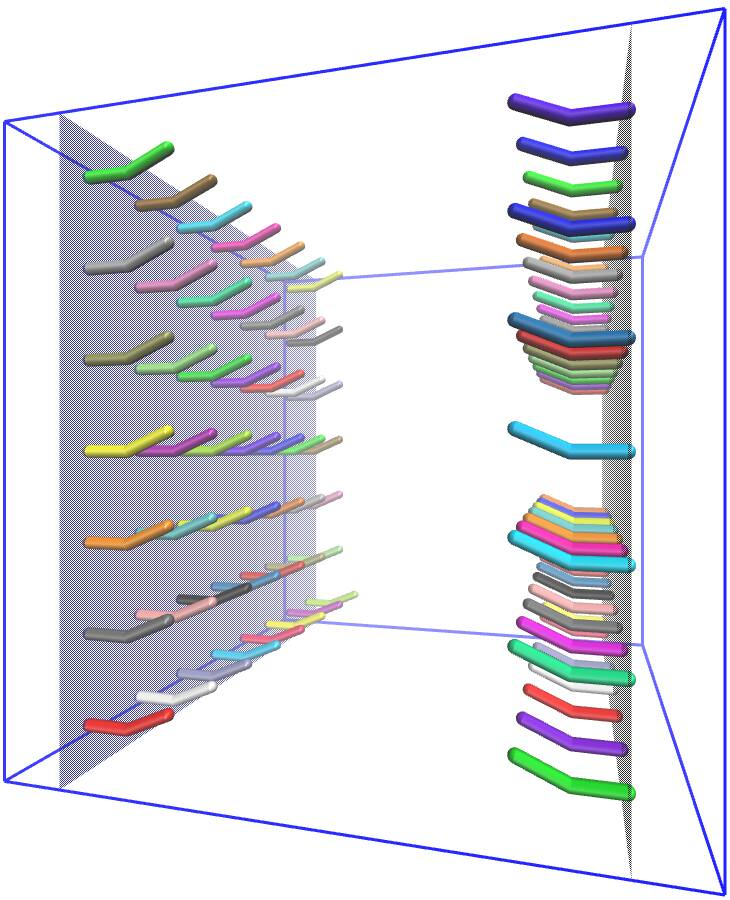
\includegraphics[angle=180,width=\textwidth]{GenLayers-478ctac.jpg}
\end{minipage}
\begin{minipage}{0.5\textwidth}
\begin{verbatim}
  10 10 10
  species 1
  A   1.0 0.0 0
  molecules 1
  A3
  nummols 1
  beads 4
  A 0 0.0 0.0
  A 0 0.0 0.7
  A 0 0.5 1.2
  A 0 0.0 1.7
  bonds 3
  harm 1 2 100 0.7
  harm 2 3 100 0.7
  harm 3 4 100 0.7
  finish
\end{verbatim}
\end{minipage}

Usage (\texttt{GenLayers} does not use standard options):

\vspace{1em}
\noindent
\texttt{GenSystem <out.vsf> <out.vcf> <options>}

\noindent
\begin{longtable}{p{0.15\textwidth}p{0.794\textwidth}}
  \toprule
  \multicolumn{2}{l}{Mandatory arguments} \\
  \midrule
  \texttt{<out.vsf>} & output \texttt{vsf} structure file \\
  \texttt{<out.vcf>} & output \texttt{vcf} coordinate file \\
  \toprule
  \multicolumn{2}{l}{Options} \\
  \midrule
  \texttt{-f <name>} & FIELD-like file (default: FIELD)\\
  \texttt{-v}        & verbose output that provides information about all
    bead and molecule types \\
  \texttt{-h}        & print help and exit \\
  \bottomrule
\end{longtable}
